 \documentclass[book.tex]{subfiles}
\begin{document}

Around the same time as the group was rejected by Nintendo, Romero was approached by Scott Miller of Apogee Software. They agreed to make \textit{Commander Keen in Invasion of the Vorticons}, to be published by Apogee Software. The team could not afford to leave their jobs to work on the game full-time, so they continued to work at Softdisk, spending their time on the Gamer's Edge games during the day and on Commander Keen at night and weekends using Softdisk computers. The game was completed in early December 1990.\\

\par
After the arrival of the first royalty check from Apogee, the team planned to quit Softdisk and start their own company. On February 1, 1991, the team founded \textit{id Software} having four owners: John Carmack, John Romero, Tom Hall and artist Adrian Carmack\footnote{See Masters of Doom, chapter 4}. \\

\par
\begin{fancyquotes}
I told them we need to start a company, do our own game and publish it, outside of Softdisk. Jay Wilbur happened by the office and I told him that after what had been done by John and Tom the night before, we were outta there. He kinda laughed and said, "Heheh, yeah..." and I said, "No. I'm serious - we're gone." Jay quickly closed the door and wanted to know what we were thinking of doing.\\
\par
\textbf{John Romero - founder of id Software.}
\end{fancyquotes}\\
\par


When their boss and owner of Softdisk, Al Vekovius, confronted them on their plans, as well as their use of company resources to develop the game, the team made no secret of their intentions. Vekovius initially proposed a joint venture between the team and Softdisk, which fell apart when the other employees of the firm threatened to quit in response, and after a few weeks of negotiation the team agreed to produce a series of games for Gamer's Edge, one every two months. One of the games they developed to fulfill their obligation was Commander Keen in Keen Dreams.\\
\par


\begin{figure}[H]
\begin{subfigure}{.5\textwidth}
  \centering
  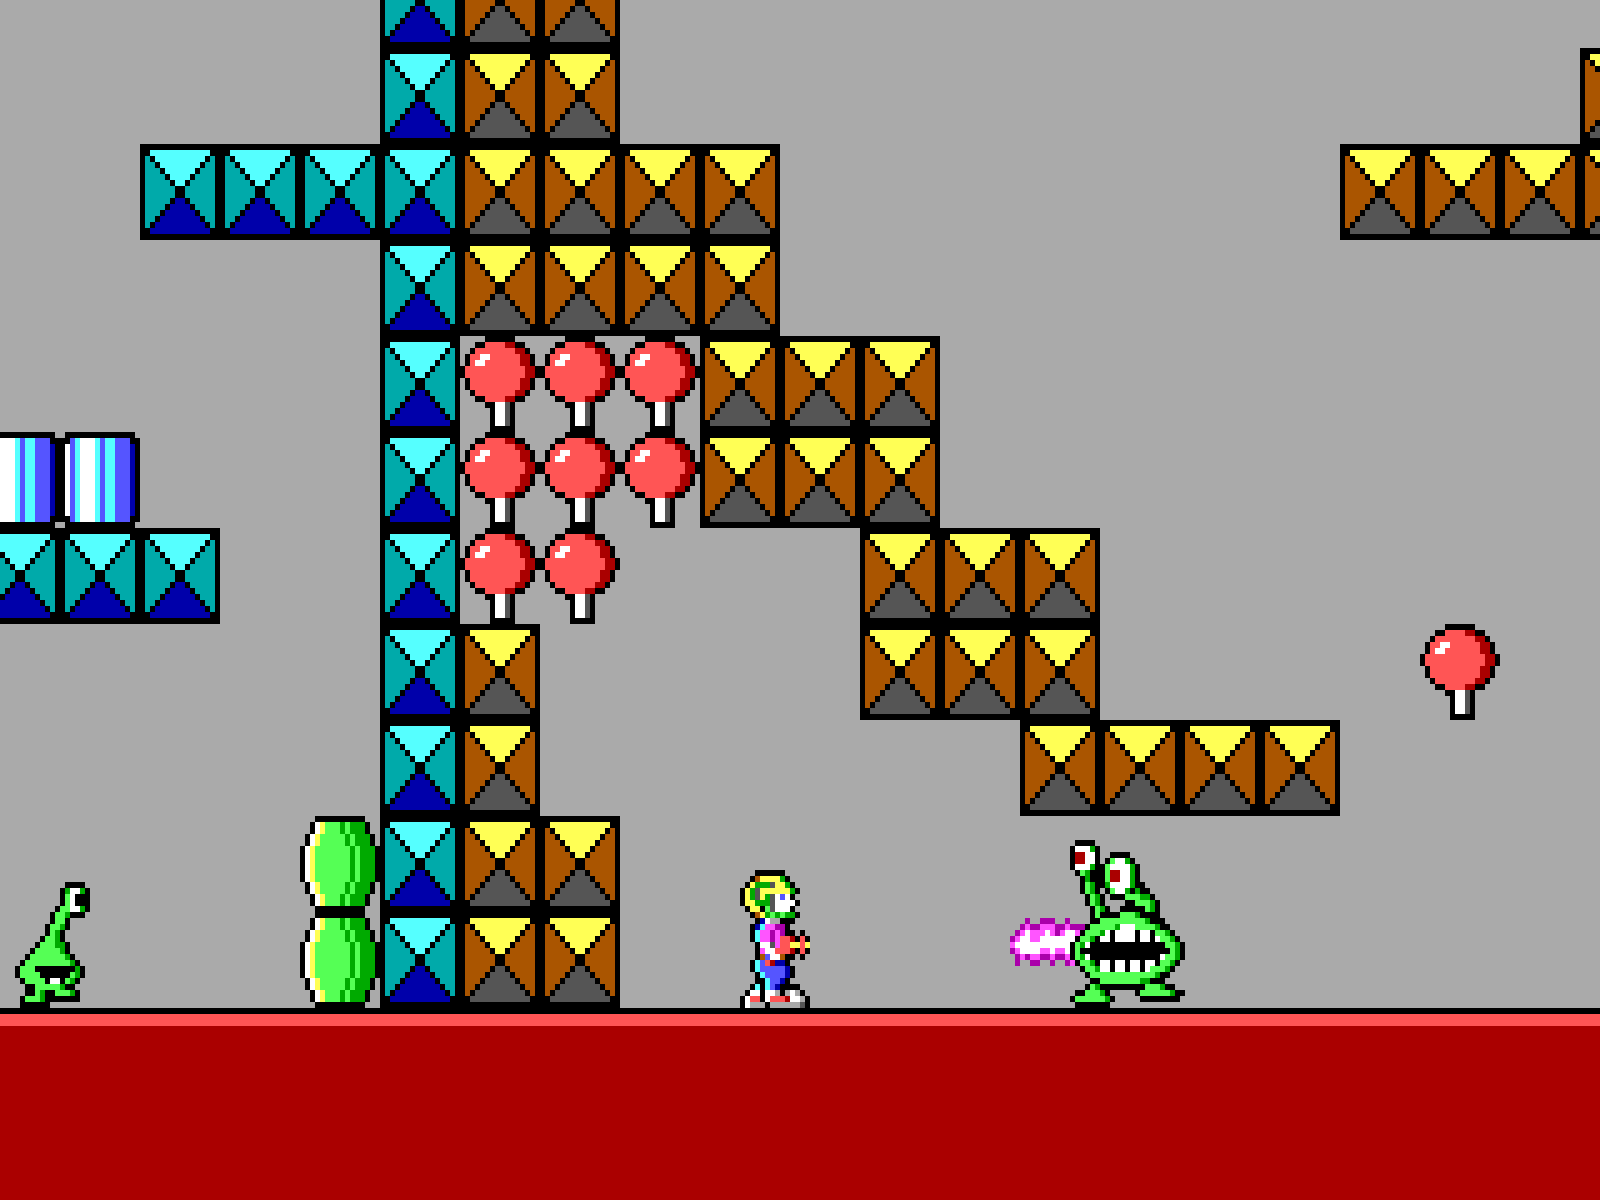
\includegraphics[width=.95\textwidth]{screenshots_300dpi/Keen_Marooned_on_Mars_gameplay.png}
  \caption*{Keen 1 - Marooned on Mars.}
\end{subfigure}%
\begin{subfigure}{.5\textwidth}
  \centering
  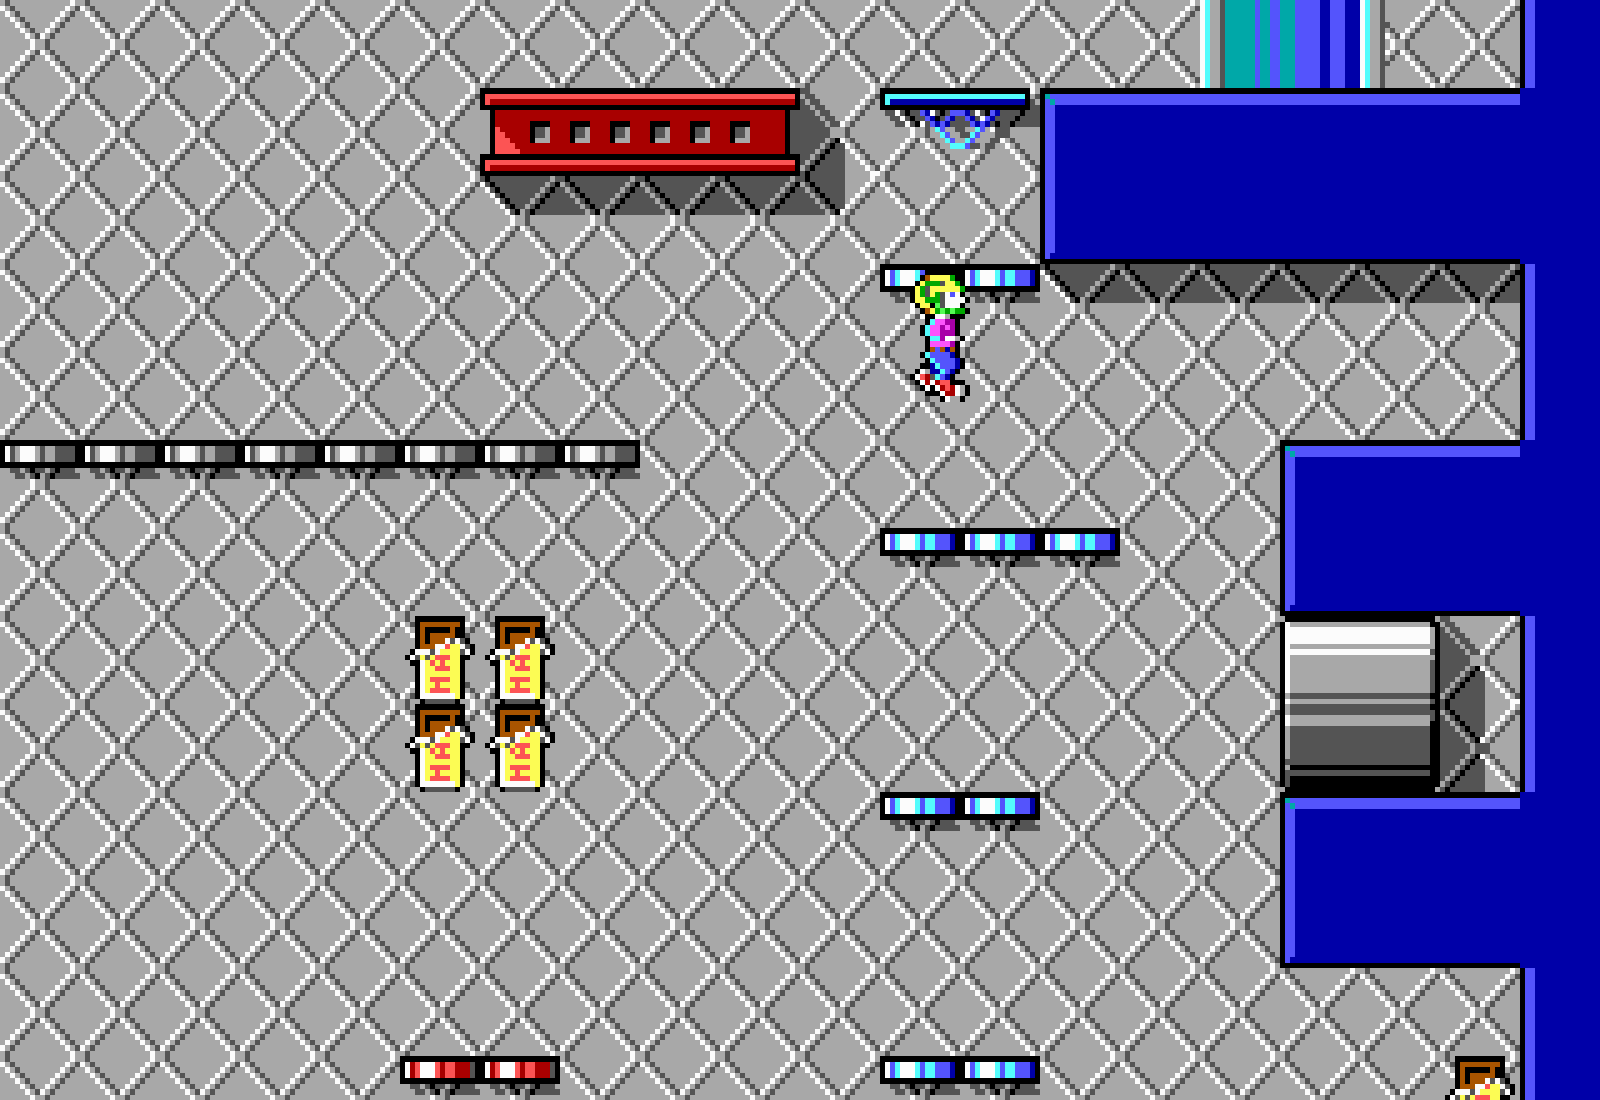
\includegraphics[width=.95\textwidth]{screenshots_300dpi/keen1_2.png}
  \caption*{Keen 2 - The Earth Explodes.}
\end{subfigure}
\par\bigskip % force a bit of vertical whitespace
\begin{subfigure}{.5\textwidth}
  \centering
  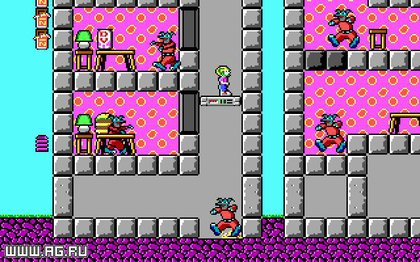
\includegraphics[width=.95\textwidth]{screenshots_300dpi/keen1_3.jpg}
  \caption*{Keen 3 - The Earth Explodes.}
\end{subfigure}
\begin{subfigure}{.5\textwidth}
  \centering
  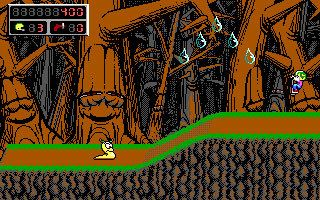
\includegraphics[width=.95\textwidth]{screenshots_300dpi/keen2_1.jpg}
  \caption*{Keen 4 - Secret of the Oracle.}
\end{subfigure}
\par\bigskip % force a bit of vertical whitespace
\begin{subfigure}{.5\textwidth}
  \centering
  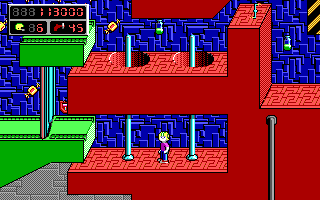
\includegraphics[width=.95\textwidth]{screenshots_300dpi/keen2_2.png}
  \caption*{Keen 5 - The Armageddon Machine.}
\end{subfigure}
\begin{subfigure}{.5\textwidth}
  \centering
  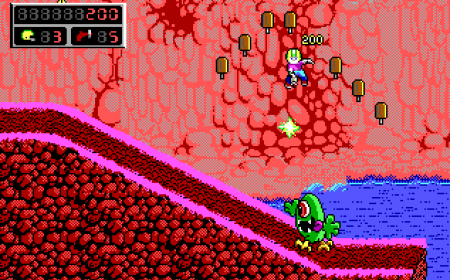
\includegraphics[width=.95\textwidth]{screenshots_300dpi/keen3_1.png}
  \caption*{Keen 6 - Aliens Ate My Babysitter.}
\end{subfigure}
\caption{Commander Keen Episode 1-6.}
\label{fig:draw_layers}
\end{figure}
\par

Between 1990 and 1991 the team published \textit{Commander Keen in Invasion of the Vorticons} and \textit{Commander Keen in Goodbye, Galaxy}, and the stand-alone games \textit{Commander Keen in Keen Dreams} and \textit{Commander Keen in Aliens Ate My Babysitter}. Another trilogy of episodes, titled \textit{The Universe Is Toast}, was planned for December 1992; id worked on it for a couple of weeks, but then shifted the work to another game. The name of that new game was \textbf{Wolfenstein 3D}...

\end{document}